%!TEX root = /Users/velrok/Dropbox/TheoInf Seminar/Ausarbeitung/Main.tex


\section{Modal-Logik ($K$)} % (fold)
\label{sec:modal_logic}

\subsection{Syntax} % (fold)
\label{sec:syntax}
Die Syntax der Modal Logik entspricht der der Aussagenlogik mit den Erweiterungen $\square$ und $\Diamond$. 
Wie die Negation sind diese unär, das heißt sie beziehen sich nur auf die ihr folgende Formel. Im Folgenden werden die Zeichen $p, q, r, p_3$ für atomare Formeln verwendet.\cite[S.307f]{huth2004logic}\\
\\
\begin{definition}
	\label{def:syntax}
	Die folgende BNF (Backus Naur Form) beschreibt die Syntax der möglichen multi modal Formeln $\phi$.

	\begin{equation}
		\label{eqn:bnf}
		\phi ::= \bot|\top|p|(\neg\phi)|(\phi\wedge\phi)|(\phi\vee\phi)|(\phi\rightarrow\phi)|
		(\phi\leftrightarrow\phi)|(\square\phi)|(\Diamond\phi)
	\end{equation}
\end{definition}
\cite[S.307]{huth2004logic}

\begin{figure}[ht]
	\begin{center}
  	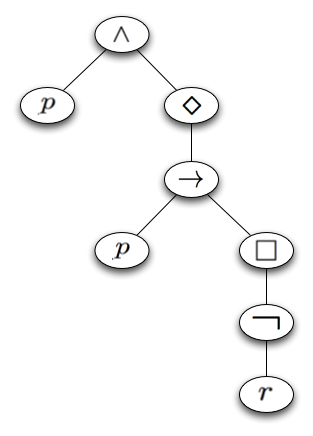
\includegraphics[width=0.4\textwidth]{./Images/mmFormel01.png}
		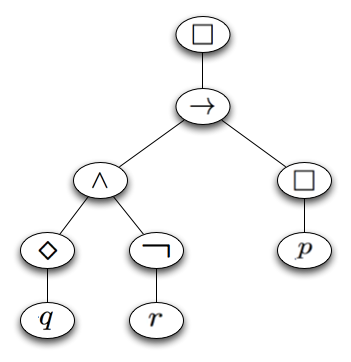
\includegraphics[width=0.4\textwidth]{./Images/mmFormel02.png}
  	\caption{Parse-Tree für $(p \wedge \Diamond(p \rightarrow \square \neg r))$ und 
		$\square((\Diamond q \wedge \neg r) \rightarrow \square p )$}
		\label{fig:mmFormel01}
	\end{center}
\end{figure}


Die Formeln $(p \wedge \Diamond(p \rightarrow \square \neg r))$ und 
$\square((\Diamond q \wedge \neg r) \rightarrow \square p )$ sind Beispiele für syntaktisch korrekte Multi-Modal-Logik Formeln. Ihre Parse-Trees sind abgebildet in Abbildung~\ref{fig:mmFormel01}.\\
\\
Wie auch bei der Aussagenlogik binden die unären Operatoren stärker als die Binären.
Sodass unnötige Klammern weggelassen werden können um die Leserlichkeit zu verbessern.\\
\\
Die folgende Liste sortieren die Operatoren nach ihrer Bindungsstärke. Beginnend mit den am stärksten bindenden.\\
\begin{itemize}
	\item $\neg, \square, \Diamond$
	\item $\wedge, \vee$
	\item $\rightarrow, \leftrightarrow$
\end{itemize}

Im allgemeinen werden die Symbole $\square$ und $\Diamond$ als Box und Raute gelesen. 
Spezifiziert man eine konkrete Logik so werden diese entsprechend ihrer interpretation gelesen. In der Logik für Notwendigkeit wird $\square$ als notwendig und $\Diamond$ als möglich gelesen. In Logik für über das Wissen eines Agenten Q, wird $\square$ als Q weis und $\Diamond$ als soweit Q weis, gelesen.


% section syntax (end)

\subsection{Semantik} % (fold)
\label{sec:semantik}

Dieses Kapitel beschreibt die Semantik von Modal-Logik-Aussagen. 
Die Semantik wird dabei formal beschrieben. Die grundlegende Frage ist wann evaluiert eine Modal-Logik-Formel zu \emph{wahr} bzw. \emph{falsch}.

Zur Erinnerung: In der Aussagenlogik ist eine Interpretation eine mögliche Belegung der Variablen mit den Wahrheitswerten \emph{Wahr} oder \emph{Falsch}. Dabei muss jeder der Variablen einen dieser Werte annehmen. Die Formel $a \wedge b$ hat $2_2 = 4$ mögliche Interpretationen. 
\begin{figure}[ht]
	\begin{center}
		\begin{tabular}{cccc}
		\hline
		a & b & $a \wedge b$\\
		\hline
		1 & 1 & Wahr\\
		\hline
		1 & 0 & Falsch\\
		\hline
		0 & 1 & Falsch\\
		\hline
		0 & 0 & Falsch\\
		\hline
		\end{tabular}
		\caption{Alle möglichen Interpretationen der Aussagenlogik-Formel $a \wedge b$}
		\label{tab:AussagenlogikInterpretation}
	\end{center}
\end{figure}
Siehe Abbildung~\ref{tab:AussagenlogikInterpretation}
\cite{hunter1973metalogic}% wikipedia: Was ist eine Interpretation http://en.wikipedia.org/wiki/First-order_logic#Evaluation_of_truth_values

Die Modal-Logik erfordert ein komplexeres Model für die Auswertung von Formeln, da verschiedene Arten von Wahr modelliert werden können.\cite[S.308f]{huth2004logic}
Ein Model in Modal-Logik wird deswegen durch eine Kripkestruktur beschrieben. 

\begin{definition}
	\label{def:model}
	Ein Model $M$ einer Modal Logik wird durch 3 Bestandteile beschrieben:
	\begin{itemize}
		\item Einer Menge von Welten $W$
		\item einer Erreichbarkeitsfunktion $R$ auf $W$ ($R \subseteq WxW$)
		\item einer \fachwort{Labelingfunktion} $L : W \rightarrow P(Atome)$
	\end{itemize}
	
	Man schreibt $R(x,y)$ um zu kennzeichnen, dass $(x,y)$ in $R$ enthalten ist.
	
\end{definition}
\cite[S.309]{huth2004logic}


Nehmen wir an die Menge der Welten $W$ sei 
\begin{center}
	$\{ x_1, x_2, x_3, x_4, x_5, x_6 \}$
\end{center}
 
die Relation $R$ sei definiert als 
\begin{center}
	$\{(x_1, x_2), (x_1, x_3), (x_2, x_3), (x_3, x_2), (x_2, x_2), (x_4, x_5), (x_5, x_4), (x_5, x_6)\}$ 
\end{center}

und die Labelfunktion $L$ liefere,
\begin{center}
	\begin{tabular}{c|cccccc}
		$x$ & $x_1$ & $x_2$ & $x_3$ & $x_4$ & $x_5$ & $x_6$\\
		\hline
		$L(x)$ & $\{q\}$ & $\{p,q\}$ & $\{p\}$ & $\{q\}$ & $\{\}$ & $\{p\}$
	\end{tabular}
\end{center}

dann ist Abbildung~\ref{fig:mmKripke01} die graphische Darstellung der beschriebenen Kripke-Struktur.

\begin{figure}[ht]
	\begin{center}
  	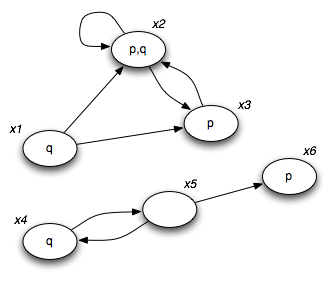
\includegraphics[width=0.65\textwidth]{./Images/Kripke01.png}
  	\caption{Beispiel einer Kripke-Struktur}
		\label{fig:mmKripke01}
	\end{center}
\end{figure}

\begin{definition}
	\label{def:reasoning}
	Sei $M = (W,R,L)$ ein Model einer Modal Logik und $\phi$ sei eine Formel nach \eqref{eqn:bnf}.
	Dann lässt sich nach folgenden Regeln schließen of $\phi$ in einer Welt $x$ \emph{Wahr} oder \emph{Falsch} ist.
	\begin{align}
	%	\begin{split}
		x &\Vdash \top\label{eqn:semanticTrue}\\
		x &\nVdash \bot\label{eqn:semanticFalse}\\
		x &\Vdash p\text{ gdw. }p \in L(x)\label{eqn:semanticLabel}\\
		x &\Vdash \neg \phi\text{ gdw. }x \nVdash \phi\\
		x &\Vdash \phi \wedge \psi\text{ gdw. }x \Vdash \phi\text{ und } x \Vdash \psi\label{eqn:semanticAnd}\\
		x &\Vdash \phi \vee \psi\text{ gdw. }x \Vdash \phi \text{, oder } x \Vdash \psi\\
		x &\Vdash \phi \rightarrow \psi\text{ gdw. }x \Vdash \psi\text{, immer wenn gilt }x \Vdash \phi\\
		x &\Vdash \phi \leftrightarrow \psi\text{ gdw. }( x \Vdash \phi\text{ gdw. }x \Vdash \psi)\label{eqn:semanticBiconditional}\\
		x &\Vdash \Box \psi \text{ gdw. }\forall y \in W \text{ gilt } R(x,y)\text{, und } y \Vdash \psi\label{eqn:semanticBox}\\
		x &\Vdash \Diamond \psi\text{ gdw. }\exists y \in W \text{ sodass }R(x,y)\text{ und }y \Vdash \psi\label{eqn:semanticDiamond}
	%	\end{split}
	\end{align}	
\end{definition}
\cite[S.310]{huth2004logic}

Die Formeln \eqref{eqn:semanticTrue} und \eqref{eqn:semanticFalse} besagt, dass die Werte \emph{wahr} und \emph{falsch} enthalten sind. 
Die Formel \eqref{eqn:semanticLabel} besagt, dass wir Aussagen folgern können die Teil der Wissensbasis sind.
Die Formeln \eqref{eqn:semanticAnd} bis \eqref{eqn:semanticBiconditional} sind ähnlich zu denen aus der Aussagenlogik.
Spannend sind die Formeln \eqref{eqn:semanticBox} und \eqref{eqn:semanticDiamond}. 
\eqref{eqn:semanticBox} besagt, dass die Aussage $\Box\psi$ für eine Welt $x$ gefolgert werden kann, wenn diese in allen Welten die von $x$ aus erreichbar sind, gefolgert werden kann. Dies beinhaltet $x$ nur wenn $R(x,x)$ gilt.
Wichtig ist das die Aussage lediglich fordert, das eine Aussage in allen \emph{erreichbaren} Welten gefolgert werden kann. $x \Vdash \Box \bot$ ist also \emph{wahr} wenn $x$ mit keiner anderen Welt verbunden ist.
Die Formel \eqref{eqn:semanticBox} ist ähnlich, nur das sie einen existenz Charakter hat. Aus $x$ lässt sich $\Diamond \psi$ folgern, wenn es min. eine Welt gibt die von $x$ erreichbar ist in der sich $\psi$ folgern lässt. Wichtig ist die Aussage es \emph{existiert} eine Welt. $x \Vdash \Diamond \top$ ist also \emph{falsch} wenn es keine Welt $x'$ gibt für die gilt $R(x,x')$.

\begin{definition}
	\label{def:model_erfuellt}
	Ein Model $M$ einer Modal Logik erfüllt eine Formal $\phi$ wenn jeder Zustand im Model die Formel erfüllt.
	Wir schreiben für diesen Fall $M \vDash \psi$ gdw. $\forall x \in W, x \Vdash \psi$
\end{definition}
\cite[S.310f]{huth2004logic}



\todo{definitionen einsortieren und mit Kontext versehen}

\textbf{Gleichheit zwischen modal logischen Formeln}
\begin{definition}
	\label{def:model_folgert}
	\begin{itemize}
		\item Eine Menge von modal logischen Formeln $\Gamma$ folgert eine modal logische Formel $\psi$, gdw. wenn für jede Welte $w$ aus jedem Model $M$ gilt: $x \Vdash \psi$ immer wenn gilt $x \Vdash \phi$ $\forall \phi \in \Gamma$. 
		Dies wird notiert durch $\Gamma \vDash \psi$.
		\item Wir bezeichnen zwei modal logische Formeln $\phi$ und $\psi$ als semantisch äquivalente wenn sowohl $\psi \vDash \phi$ als auch $\psi \vDash \phi$ gilt.
	\end{itemize}	
\end{definition}
\cite[S.313]{huth2004logic}

\textbf{valide Formeln}
\begin{definition}
	\label{def:valide}
	Eine modal logische Formel $\psi$ wird valide genant wenn sie in jeder Welt in jedem Model \emph{Wahr} ist, also gdw. $\vDash \psi$ gilt.
\end{definition}
\cite[S.314]{huth2004logic}


\textbf{Ähnlichkeitstheorie}
\begin{definition}
	\label{def:frame}
	Ein Frame $F = (W,R)$ ist eine Menge von Welten $W$ und eine binäre Relation $R$ auf $W$.
\end{definition}
\cite[S.322]{huth2004logic}
\note{labeling funktion fehlt}


\begin{definition}
	\label{def:frame_erfuellt}
	Ein Frame $F$ erfüllt eine modal logische Formal $\psi$, wenn für jede \fachwort{Labelfunktion} $L: W \rightarrow P(Atome)$ und jedes $w \in W$, es der Fall ist, dass $M,w \vDash \psi$ gilt. $M$ ist das Model: $M = (W,R,L)$.
	In diesem Falle schreiben wir $F \vDash \psi$.
\end{definition}
\cite[S.322f]{huth2004logic}
\todo{entsprechende Buchstaben in MathDS auszeichnen}

\textbf{einige Modal Logiken}
\begin{definition}
	\label{def:substitution}
	Sei $\mathds{L}$ eine Menge von Formel-Schemata der Modal Logik und $\Gamma \cup {\psi}$ eine Menge von modal logischen Formeln.
	
	\begin{itemize}
		\item Die Menge $\Gamma$ ist abgeschlossen gegenüber der Substitution von Instancen gdw.  $\psi \in \Gamma$. Dann gilt auch, dass jede Substitutionsinstanz von $\psi$ auch in $\Gamma$ ist.
		\item Sei $\mathds{L}_c$ die kleinste Menge die alle Instanzen von $\mathds{L}$ enthält.
		\item Aus $\Gamma$ folgt semantisch $\psi$ in $\mathds{L}$ gdw. alle Modelle, deren Frame $\mathds{L}$ erfüllt und alle Welten $x$ in diesem Modell, $x$ erfüllt $\Gamma$, gilt.
		In diesem Fall sagen wir $\Gamma \vDash_{\mathds{L}} \psi$ ist erfüllt.
	\end{itemize}
\end{definition}
\cite[S.326]{huth2004logic}

\begin{definition}
	Ein Modell der intuitionistischen Aussagenlogik ist ein Model $\mathds{M} = (W,R,L)$ der Logik $KT45$, sodass $R(x,y)$ immer $L(x) \subseteq L(y)$ impliziert.
	Gegeben einer modal logische Formel nach \eqref{eqn:bnf}, definieren wir $x \Vdash \psi$ wie in Definition \eqref{def:reasoning} mit Außnahme der Reglen für $\rightarrow$ und $\neg$.
	\begin{itemize}
		\item $\psi \rightarrow \phi$ definierten wir als $x \Vdash \psi \rightarrow \phi$ gdw. $\forall y R(x,y)$ auch $y \Vdash \phi$ gilt, immer wenn $y \Vdash \psi$ gilt.
		\item $\neg \psi$ definierten wir als $x \Vdash \neg \psi$ gdw. $\forall y R(x,y)$ $y \nVdash \psi$ der Fall ist.
	\end{itemize}
\end{definition}
\cite[S.328]{huth2004logic}

\begin{definition}
	Gegeben einer Menge von Formel Schemata $\mathds{L}$.
	Definieren wir $\Gamma \Vdash_\mathds{L} \psi$ als valide, wenn es einen Beweis im natürlichen Folgerungssystem für modal Logiken gibt, der um die Axiome in $\mathds{L}$ und den Annahmen in $\Gamma$ erweitert ist.
	\todo{bessere Forumlierung finden}
	\todo{natural deduction system beser übersetzen}
\end{definition}
\cite[S.330]{huth2004logic}

\textbf{multi agent systeme}
\begin{definition}
	\label{def:bnf_kt45n}
	Eine Formel $\psi$ der multi modal Logik $KT45^n$ ist definiert durch folgende Grammatik:
	\begin{equation}
		\label{eqn:bnf_kt45n}
		\phi ::= \bot|\top|p|(\neg\phi)|(\phi\wedge\phi)|(\phi\vee\phi)|(\phi\rightarrow\phi)|
		(\phi\leftrightarrow\phi)|(K_i\psi)|(E_G\psi)|(C_G\psi)|(D_G\psi)
	\end{equation}
\end{definition}
\cite[S.335f]{huth2004logic}

\begin{definition}
		Gegeben ein Model $\mathds{M} = (W,(R_i)_{i \in \mathds{A}}, L)$ der $KT45^n$ und eine Welt $w \in W$, so definieren $\psi$ als \emph{Wahr} durch die Erfüllung der Relation $x \vDash \psi$ durch folgende Regeln:
		\begin{align}
			x &\Vdash p\text{ gdw. }p \in L(x)\\
			x &\Vdash \neg \phi\text{ gdw. }x \nVdash \phi\\
			%
			x &\Vdash \phi \wedge \psi\text{ gdw. }x \Vdash \phi\text{ und } x \Vdash \psi\\
			x &\Vdash \phi \vee \psi\text{ gdw. }x \Vdash \phi \text{, oder } x \Vdash \psi\\
			%
			x &\Vdash \phi \rightarrow \psi\text{ gdw. }x \Vdash \psi\text{, immer wenn gilt }x \Vdash \phi\\
			%
			x &\Vdash K_i\psi \text{ gdw. } \forall y \in W, R_i(x,y) \text{, } y \Vdash \psi \text{ impliziert}\\
			x &\Vdash E_G\psi \text{ gdw. } \forall i \in G, x \Vdash K_i\psi\\
			x &\Vdash C_G\psi \text{ gdw. } \forall k \geq 1 \text{, und es gilt } x \Vdash E^k_G\psi \text{.} \text{Wobei } E^k_G \text{ meint } E_{G}E_{G}\dots E_{G} \text{ k-mal.}\\
			x &\Vdash D_G\psi \text{ gdw. } \forall y \in W, y \Vdash \psi \text{gilt, immer wenn auch } R_i(x,y), \forall i \in G \text{gilt.}\\
		\end{align}
\end{definition}
\cite[S.337]{huth2004logic}



























% section semantik (end)

\subsection{Attribute einer Modal-Logik} % (fold)
\label{sub:attribute_einer_modal_logik}
Die Attribute einer Modal-Logik beschreibt welche Formel-Schemata diese Logik beinhaltet. Daraus lassen sich wiederum Eigenschaften der Wahrheitsmodalität ableiten. 
Will man eine eigene Modal-Logik kreieren ist es wichtig sich genaue Gedanken darüber zu machen, welcher dieser Eigenschaften auf die zu kreierende Logik-Modalität zutreffen sollen.
Im Folgenden wird erst das für Normale Logiken zwingend erforderliche Basisattribut $K$ vorgestellt und danach auf die anderen optionalen Eigenschaften eingegangen. 
Zum Schluss werden ein paar Modal-Logiken und deren Eigenschaften beschrieben und erklärt, warum die gewählten Eigenschaften für die Modalität wünschenswert / wichtig / notwendig sind.
Es gibt auch \fachwort{Nicht Normale Modallogik}en

\paragraph{Das Basis Atribute $K$} % (fold)
\label{par:das_basis_atribute_k_} $p \wedge (p \rightarrow q) \rightarrow q$ besagt das die Logik geschlossen ist unter der logischen Konsequentz. \todo{mehr schreiben}

\paragraph{Weitere Attribute} % (fold)
\label{par:weitere_attribute} 
\todo{weiter Atribute diskutieren}

% paragraph abgesehen_davon_gibt_es_weitere_attribute (end)
% paragraph das_basis_atribute_k_ (end)
% subsection attribute_einer_modal_logik (end)

\subsection{Ähnlichkeitstheorie} % (fold)
\label{sub:Aehnlichkeitstheorie}
Die Ähnlichkeitstheorie besagt, das sich die Eigenschaften einer Modal-Logik in der Relation der entsprechenden Kripkestrucktur widerspiegeln und vis versa. 
Dies schafft einen neuen Zugang zum Design von Modal-Logiken. 
In manchen Fällen mag es einfacher sein in den notwendigen Eigenschaften in Form von Formel-Schemata zu denken, in anderen ist es evtl. einfacher das Problem über die Relation zu verstehen. 
Im Folgenden wird gezeigt, wie die einzelnen Eigenschaften mit der Kripke-Struktur-Relation zusammen hängen.

\todo{mehr schreiben}

% subsection Aehnlichkeitstheorie (end)

% section basic_modal_logic (end)

\subsection{Die Modal-Logik $KT45$ (Wissen)} % (fold)
\label{sub:the_normal_modal_logic_s5_}

% subsection the_normal_modal_logic_s5_ (end)